
%% MAIN FILE
%% This is the file which you compile with LaTeX

%% INSTRUCTIONS
%%      The places marked with ACTION, require your action
%%      The places marked with OPTIONAL, highlight key places where action can be taken
%%      Other comments are left to provide for those who wish to modify the template

%% Comments with '%% ...' are comments
%% Comments with '% ...' are deactivated code, which you may wish to uncomment


%%********************************************************************************
%% Core headers
%%****************************************
%% Using the class Thesis.cls, which is included with this template
%% Thesis.cls has been modified by many, based on the ECS Thesis style originally by Steve Gunn
\documentclass{Thesis}

%% Font Choice
%\usepackage[lining]{nunito}


%%********************************************************************************
%% Embed pdfs (part 1)
%%****************************************
\usepackage{pdfpages} %% Embed pdfs


%%********************************************************************************
%% Embed pdfs (part 2) (OPTIONAL)
%%****************************************
%% TO USE: Manual actions are required. See instructions below
%% TO SKIP: No action required. Leave everything as is or comment it out

%% PURPOSE
%%      By using the package `pdfpages' to embed this pdf into the thesis, all the hyperlinks become no longer clickable.
%%      To reinsert the links, the package `pax' can be used

%% INSTRUCTIONS
%%      Stage 1 (only needs to be run once)
%%      Compile with LuaLaTeX
%%      Then Rename the output files from *.newpax to *.pax
%%      For me, some of the links were broken. Either delete them from the pax file, or manually fix them in the pax file
%%      Stage 2 (run on every compile)
%%      Compile with pdflatex as normal
%% Notes
%%      For stage 1, the file extension should not be included
%%      Stage 2 doesn't like the pdfs sitting in subfolders

%% (STAGE 1) Extract links
\usepackage{ifluatex,etoolbox}
\ifluatex
    \directlua{require("newpax")}
    \directlua{
        newpax.writenewpax("MyPublishedArticle1")
        newpax.writenewpax("MyPublishedArticle2")
    }
\fi

%% (STAGE 2) Insert links
%% newpax requires the package pdfmanagement-testphase
%% But this is not compatible with the pdfx package
%% => Using the output of nexpax with pax
%% The following is copied from the newpax documentation
\ifluatex
    \usepackage{pdftexcmds}
    \makeatletter
    \let\pdfstrcmp\pdf@strcmp
    \let\pdfescapename\pdf@escapename
    \makeatother
    \usepackage{luatex85}
\fi
\usepackage{pax}
%% Correct a bug in pax affecting clipping
\makeatletter
\patchcmd\PAX@pdf@annot{\PAX@pagellx}{\PAX@page@llx}{}{\fail}
%% Allow hashes and percent in the pax file
\patchcmd\PAX@AddAnnots{\InputIfFileExists\PAX@file{}{\typeout{* Missing: \PAX@file}}}
{\begingroup \catcode`\#=12 \catcode`\%=12
\InputIfFileExists\PAX@file{}{\typeout{* Missing: \PAX@file}}\endgroup}{}{\fail}
\makeatother


%%********************************************************************************
%% Tables (required for the table in Preamble/Declaration_publications.tex)
%%****************************************
\usepackage{silence}
\WarningFilter{latex}{You have requested package `lib/nicematrix',} %% Using local as the latest version is not avaliable on overleaf
\usepackage{lib/nicematrix} %% Tables, matrices, etc.


%%********************************************************************************
%% Bibliography
%%****************************************
\usepackage[style=numeric, sorting=none, isbn=false, url=true,sortcites=true,maxbibnames=99]{biblatex}
\renewcommand*{\bibfont}{\small}

%% Prevent "et al." in \fullcite https://tex.stackexchange.com/a/267089
\preto\fullcite{\AtNextCite{\defcounter{maxnames}{99}}}

%% ACTION: Include your references in the .bib file
\addbibresource{Bibliography/Bibliography.bib}


%%********************************************************************************
%% OPTIONAL: Add your own packages and commands here
%%****************************************


%%%%%%%%%%%%%%%%%%%%%%%%%%%%%%%%%%%%%%%%%%%%%%%%%%%%%%%%%%%%%%%%%%%%%%%%%%%%%%%%%
%% Start
%%%%%%%%%%%%%%%%%%%%%%%%%%%%%%%%%%%%%%%%%
\begin{document}

%% ACTION: Add your details here
%%      These are used in the title page, preliminary pages, and pdf metadata
\thesisUniversity{Monash University}
\thesisSchool{My Faculty}
\thesisDepartment{My Department} %% 'Department of ...' / 'School of ...'
\thesisGradtime{year} %% Year of thesis submission
\thesisDegree{Doctor of Philosophy} %% `Doctor of Philosophy' or `Master of ...'
\thesisPriorDegrees{My previous academic degrees}
\thesisTitle{My Thesis Title is Long:\\So I added A Line Break For Style}
\thesisAuthor{My Full Name}

%% ACTION: Add your details here
%%      The following are used in the pdf's metadata only
%%      Use the exact formatting, otherwise other programs won't recognise it.
\thesisPublicationType{phdthesis} %% Use a Bibtex entry type `phdthesis' or `mastersthesis'
\thesisLanguage{en-AU} %% Use an `IETF language tag' https://en.wikipedia.org/wiki/IETF_language_tag

\makemetadata
\maketitle


%%%%%%%%%%%%%%%%%%%%%%%%%%%%%%%%%%%%%%%%%%%%%%%%%%%%%%%%%%%%%%%%%%%%%%%%%%%%%%%%%
%%%%%%%%%%%%%%%%%%%%%%%%%%%%%%%%%%%%%%%%%%%%%%%%%%%%%%%%%%%%%%%%%%%%%%%%%%%%%%%%%
%% Header/footer style
\frontmatter %% Begin Roman style (i, ii, iii, iv...) page numbering
\assignpagestyle{\chapter}{preliminarypages}
\pagestyle{preliminarypages}

%% OPTIONAL
%%      Line-spacing: I suggest that all 3 commands have the same value
\setstretch{1.3} %% Normal text
\captionsetup{font={stretch=1.3}} %% Figures
\captionsetup[sub]{font={stretch=1.3}} %% SubFigures

%% ACTION
%%      Update each of the preliminary pages
% https://www.monash.edu/graduate-research/examination/publication
% https://www.monash.edu/rlo/graduate-research-writing/write-the-thesis
% https://www.monash.edu/rlo/graduate-research-writing/write-the-thesis/writing-the-thesis-chapters/structuring-a-long-text
\copyrightnotice{

% \addtocontents{toc}{\vspace{1em}}  % Add a gap in the Contents, for aesthetics

\emph{Insert one of the following notices.}

\emph{Notice 1}

\textsuperscript{\textcopyright  \authornames (\gradtime).}

\emph{The second notice certifies the appropriate use of any third-party material in the thesis. Students choosing to deposit their thesis into the restricted access section of the repository are not required to complete Notice 2.}

\emph{Notice 2}

\textsuperscript{\textcopyright  \authornames (\gradtime).}

I certify that I have made all reasonable efforts to secure copyright permissions for third-party content included in this thesis and have not knowingly added copyright content to my work without the owner's permission.


}
% https://www.monash.edu/graduate-research/examination/publication
% https://www.monash.edu/rlo/graduate-research-writing/write-the-thesis
% https://www.monash.edu/rlo/graduate-research-writing/write-the-thesis/writing-the-thesis-chapters/structuring-a-long-text
\abstract{
\addtocontents{toc}{}  % Add a gap in the Contents, for aesthetics

\emph{The abstract should outline the main approach and findings of the thesis and must not be more than 500 words.}

}

%% (OPTIONAL)
%% Publications during enrolment
%% ACTION
%%      You may wish to list your publications arising from your research degree enrolment. Otherwise remove this section.
%%      The format of this section is mostly up to you. I have added lists for categorisation by type. You may alter this.
\Publicationslist{{}
Journal Publications\\[-3\parskip]
{\small
\begin{itemize}
	\item \fullcite{example3}
	\item \fullcite{example5}
\end{itemize}
}

Conference Publications\\[-3\parskip]
{\small
\begin{itemize}
	\item \fullcite{example1}
	\item \fullcite{example2}
\end{itemize}
}

Research Data\\[-3\parskip]
{\small
\begin{itemize}
	\item \fullcite{example4}
\end{itemize}
}

%% SYNTAX: \href{ref}{text}
%% NOTE: Escape underscores in the displayed text with \_ (the ref should just be the url, as is)
Free \& Open Source Code\\[-3\parskip]
{\small
\begin{itemize}
	\item \href{https://github.com/Brandon-Johns/crane-dynamics-simulator/}{https://github.com/Brandon-Johns/crane-dynamics-simulator}
\end{itemize}
}

}
%% (REQUIRED) (Thesis including published works only)
%% ACTION
%%      Ensure that your thesis meets the thesis including published works requirements. Some faculties vary requirements in terms of the number of papers required, status of papers and other criteria
%%      Read through and change the details that are in all caps (you should not use all caps in the replacement text)
\Declarationpublication{{}
I hereby declare that this thesis contains no material which has been accepted for the award of any other degree or diploma at any university or equivalent institution and that, to the best of my knowledge and belief, this thesis contains no material previously published or written by another person, except where due reference is made in the text of the thesis.

%% ACTION: Change COUNT, COUNT, THEME, NAME, NAME
This thesis includes COUNT original papers published in peer reviewed journals and COUNT submitted publications.. The core theme of the thesis is THEME. The ideas, development and writing up of all the papers in the thesis were the principal responsibility of myself, the student, working within the \printThesisDepartment under the supervision of NAME and NAME.

%% ACTION: Remove this paragraph for theses with sole-authored work
The inclusion of co-authors reflects the fact that the work came from active collaboration between researchers and acknowledges input into team-based research.

%% ACTION: If this is a laboratory-based discipline, a paragraph outlining the assistance given during the experiments, the nature of the experiments and an attribution to the contributors could follow.

%% ACTION: Insert chapter numbers
In the case of Chapters \ref{chap:article1} and \ref{chap:article2}, my contribution to the work involved the following:

%% ACTION: Update the table to list your publications
%%      The status might be: in press, accepted, returned for revision, submitted
%%      If no co-authors, leave fields blank 
\definecolor{thesisdark}{HTML}{1E1E1E}
\definecolor{thesislight}{HTML}{EEEEEE}
\newcommand{\thesisDPFormatVspace}[1]{\vspace{1ex}{#1}\vspace{1ex}}
\newcommand{\thesisDPFormatH}[1]{\textcolor{thesislight}{\textbf{#1}}}
\newcommand{\thesisDPFormatHv}[1]{\thesisDPFormatVspace{\textcolor{thesislight}{\textbf{#1}}}}
\newcommand{\thesisDPAuthorFirst}[1]{\Block[v-center]{1-1}{\thesisDPFormatVspace{#1}}}
\newcommand{\thesisDPAuthor}[1]{\cline{5-6}&&&&\Block[v-center]{1-1}{\thesisDPFormatVspace{#1}}}
\newcommand{\thesisDPAuthorYN}[1]{\Block[v-center]{1-1}{#1}\\}
\newcommand{\thesisDP}[2]{\Block[v-center]{#1-1}{#2} &}
\newcommand{\thesisDPv}[2]{\Block[v-center]{#1-1}{\thesisDPFormatVspace{#2}} &}
\begin{center}
    \addtolength{\leftskip} {-1cm} %% Fix centering for when table is wider than \textwidth
    \addtolength{\rightskip}{-1cm} %% Fix centering for when table is wider than \textwidth
    \small
    %\footnotesize
    \begin{NiceTabular}[colortbl-like]
            {|c|p{30mm}|c|p{25mm}|p{37mm}|p{25mm}|}
        \hline
        \Block[fill=thesisdark,v-center]{1-1}{\thesisDPFormatH{\makecell{Thesis\\Chapter}}} &
        \Block[fill=thesisdark,v-center]{1-1}{\thesisDPFormatH{Publication Title}} &
        \Block[fill=thesisdark,v-center]{1-1}{\thesisDPFormatH{Status}} &
        \Block[fill=thesisdark,v-center]{1-1}{\thesisDPFormatH{Nature and \% Student Contribution}} &
        \Block[fill=thesisdark,v-center]{1-1}{\thesisDPFormatHv{Co-author name(s) Nature and \% of Co-author's contribution}} &
        \Block[fill=thesisdark,v-center]{1-1}{\thesisDPFormatH{Co-author(s), Monash student}}\\

        %% ACTION: The first argument of \thesisDP must be the total number of co-authors
        %%    i.e. change the number 4 to the number of co-authors
        %%    This defines how big the multi-row block is
        \hline
        \thesisDP{4}{\ref{chap:article1}}
        \thesisDPv{4}{The Title of My First Published Article}
        \thesisDP{4}{Published}
        \thesisDP{4}{(70\%)}
        \thesisDPAuthorFirst{NAME: contribution~1, contribution~2 (10\%)} & \thesisDPAuthorYN{No}
        \thesisDPAuthor{NAME: contribution~1, contribution~2 (10\%)} & \thesisDPAuthorYN{No}
        \thesisDPAuthor{NAME: contribution~1 (5\%)} & \thesisDPAuthorYN{No}
        \thesisDPAuthor{NAME: contribution~1 (5\%)} & \thesisDPAuthorYN{No}

        %% ACTION: The first argument of \thesisDP must be the total number of co-authors
        \hline
        \thesisDP{2}{\ref{chap:article2}}
        \thesisDPv{2}{The Title of My Second Published Article}
        \thesisDP{2}{In Press}
        \thesisDP{2}{(80\%)}
        \thesisDPAuthorFirst{NAME: contribution~1, contribution~2 (10\%)} & \thesisDPAuthorYN{No}
        \thesisDPAuthor{NAME: contribution~1, contribution~2 (10\%)} & \thesisDPAuthorYN{No}
        \hline
    \end{NiceTabular}
\end{center}

I have not renumbered sections of submitted or published papers in order to generate a consistent presentation within the thesis.

\textbf{Student name:} \printThesisAuthor

%% OPTIONAL: Choose how to display the date
%%      For more options, see the package 'datetime'
\ddmmyyyydate
%\yyyymmdddate\renewcommand{\dateseparator}{-}

%% ACTION: Add your signature file
\textbf{Student signature:}\hspace{3mm}%%
\raisebox{-.5\height}{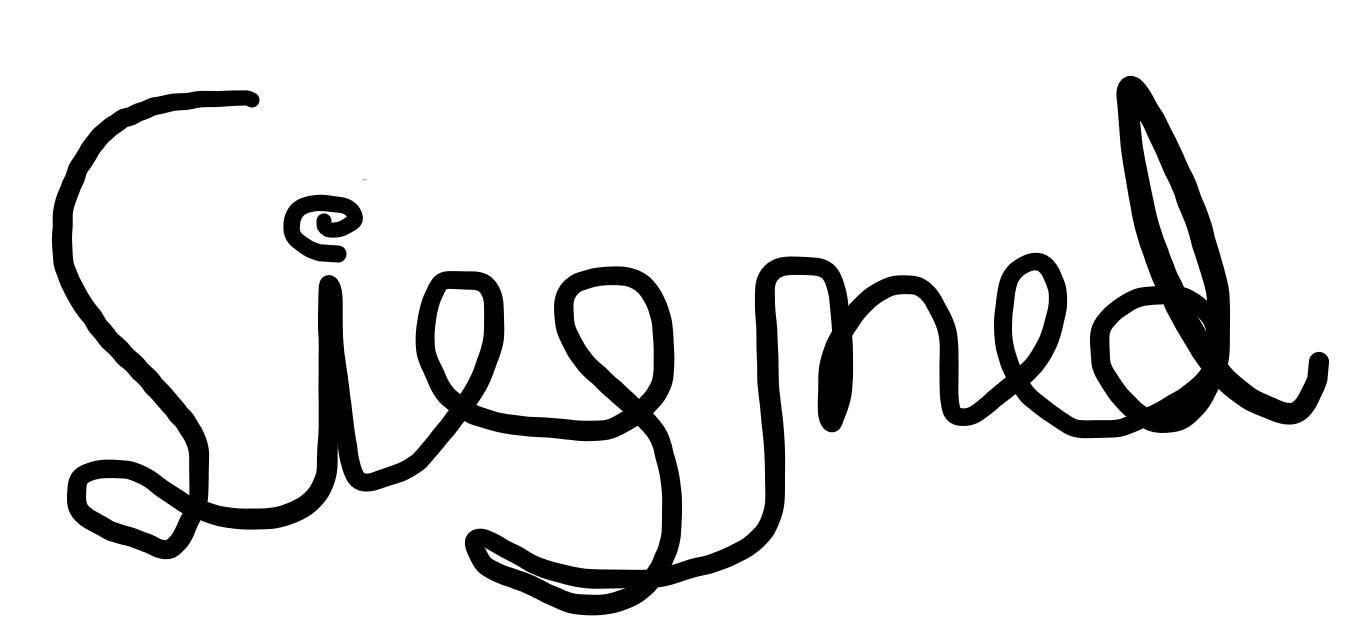
\includegraphics[height=2.5em,keepaspectratio]{Figures/SignatureMe.png}}%%
\hfill%%
\textbf{Date:} \today

I hereby certify that the above declaration correctly reflects the nature and extent of the student's and co-authors' contributions to this work. In instances where I am not the responsible author I have consulted with the responsible author to agree on the respective contributions of the authors.

%% ACTION: Add your main supervisor's name and signature file
\textbf{Main Supervisor name:} NAME

\textbf{Main Supervisor signature:}\hspace{3mm}%%
\raisebox{-.5\height}{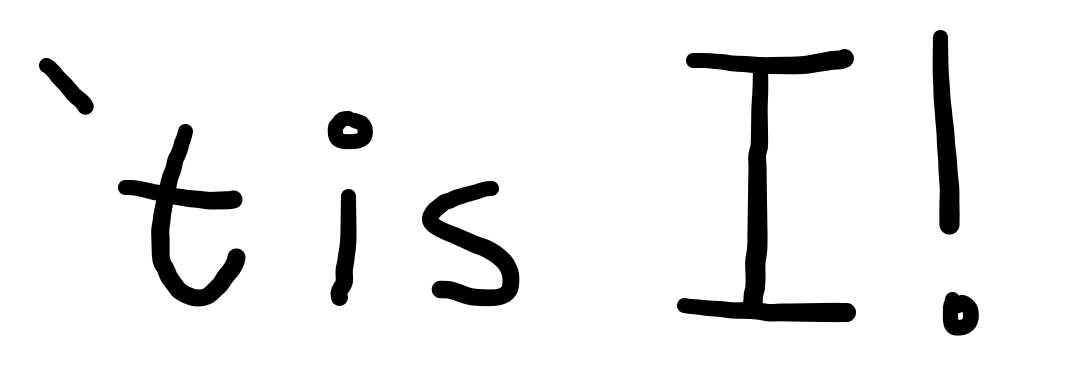
\includegraphics[height=2.5em,keepaspectratio]{Figures/SignatureSupervisor.png}}%%
\hfill%%
\textbf{Date:} \today


}
%% (REQUIRED)
%% ACTION
%%      Acknowledge your funding sources e.g. scholarships, grants
%%      The format of this section is mostly up to you. I have added a rough outline. You may alter this.
\ack{{}
Thank you to everyone who has supported me\footnote{\printThesisAuthor \href{https://orcid.org/0000-0000-0000-0000}{
\includegraphics[height=2ex]{Figures/ORCIDiD_iconvector.pdf} https://orcid.org/0000-0000-0000-0000}} during my candidature.

NAME\footnote{NAME \href{https://orcid.org/0000-0000-0000-0000}{
\includegraphics[height=2ex]{Figures/ORCIDiD_iconvector.pdf} https://orcid.org/0000-0000-0000-0000}} \textbf{---} My main supervisor. Thanks for being a great supervisor!

NAME\footnote{NAME \href{https://orcid.org/0000-0000-0000-0000}{
\includegraphics[height=2ex]{Figures/ORCIDiD_iconvector.pdf} https://orcid.org/0000-0000-0000-0000}} \textbf{---} My 2nd supervisor. Thanks for being a great supervisor!


This research was supported by an Australian Government Research Training Program (RTP) Scholarship.





}

%% ACTION
%%      Comment out any of the following to remove the section
%%      Otherwise, update the abbreviations, constants, etc.

\tableofcontents

\listoffigures

\listoftables

\listOfAbbreviations{ll}{
    \textbf{BIM} & Building Information Modelling\\
    \textbf{CAD} & Computer Aided Design\\
    \textbf{DAE} & Differential Algebraic Equation\\
    \textbf{DOF} & Degrees of Freedom\\
    \textbf{IMU} & Inertial Measurement Unit\\
    \textbf{LiDAR} & Light Detection and Ranging\\
    \textbf{NIR} & Near Infrared\\
    \textbf{ODE} & Ordinary Differential Equation\\
}

\listOfConstants{lrcl}{
    Speed of Light & $c$ & $=$ & $2.997\ 924\ 58\times10^{8}\ \mbox{ms}^{-2}$\\
}

\listOfNomenclature{lll}{%% symbol & name & unit
    $a$ & distance & m \\
    $P$ & power & W (Js$^{-1}$) \\
    & & \\
    $\omega$ & angular frequency & rads$^{-1}$ \\
}


%%%%%%%%%%%%%%%%%%%%%%%%%%%%%%%%%%%%%%%%%%%%%%%%%%%%%%%%%%%%%%%%%%%%%%%%%%%%%%%%%
%%%%%%%%%%%%%%%%%%%%%%%%%%%%%%%%%%%%%%%%%%%%%%%%%%%%%%%%%%%%%%%%%%%%%%%%%%%%%%%%%
%% Header/footer style
\mainmatter %% Begin normal, numeric (1,2,3...) page numbering
\assignpagestyle{\chapter}{corefirst}
\pagestyle{core}
\renewcommand{\chaptermark}[1]{ \markboth{\ $\vert$\ #1}{\thesubsection} }
\renewcommand{\sectionmark}[1]{ \markright{\thesubsection} }
\renewcommand{\subsectionmark}[1]{ \markright{\thesubsection} }
\renewcommand{\subsubsectionmark}[1]{}
\renewcommand{\paragraphmark}[1]{}
\renewcommand{\subparagraphmark}[1]{}


%% OPTIONAL
%% Line-spacing, if you want different line-spacing from the preliminary pages
%% I suggest that all 3 commands have the same value
%\setstretch{1.3} %% Normal text
%\captionsetup{font={stretch=1.3}} %% Figures
%\captionsetup[sub]{font={stretch=1.3}} %% SubFigures

%% ACTION
%%      The format of the chapters is up to you. I have added a rough outline and example content. You may alter this.
%%      Add your content to the chapters
%%      Delete any unused chapters
\chapter{Example Content}
This section showcases the way I formatted my lists, tables, equations, etc. If you decide to do it differently, then you'll be on your own to debug any subsequent formatting problems.

The structure of this chapter is as follows: \secref{sec:mySection} showcases the use of SSSSR sections. \secref{sec:LineBreaks} discusses the use of line breaks in section headings. \secref{sec:ContentTypes} shows how to display many different types of content.


%%%%%%%%%%%%%%%%%%%%%%%%%%%%%%%%%%%%%%%%%%%%%%%%%%%%%%%%%%%%%%%%%%%%%%%%%%%%%%%%%
%%%%%%%%%%%%%%%%%%%%%%%%%%%%%%%%%%%%%%%%%%%%%%%%%%%%%%%%%%%%%%%%%%%%%%%%%%%%%%%%%
\section{Displaying Sections} \label{sec:mySection}
This section has many subsections, which I can refer to by their labels. e.g. \secref{sec:mySection}, \secref{ssec:mySubsection}, \secref{sssec:ShinySmilyStory}, \secref{ssssec:SSSSGridman}, \secref{sssssec:Snake}, and \secref{ssec:SuperSuperRareBotan}.

Labeling sections is optional. Labels may be anything, but must be unique (hence my naming convention).

Example text.


%%%%%%%%%%%%%%%%%%%%%%%%%%%%%%%%%%%%%%%%%%%%%%%%%%%%%%%%%%%%%%%%%%%%%%%%%%%%%%%%%
\subsection{My Subsection} \label{ssec:mySubsection}
Example text.


%%%%%%%%%%%%%%%%%%%%%%%%%%%%%%%%%%%%%%%%%%%%%%%%%%%%%%%%%%%%%%%%%%%%%%%%%%%%%%%%%
\subsubsection{My Subsubsection} \label{sssec:ShinySmilyStory}
Example text.


%%%%%%%%%%%%%%%%%%%%%%%%%%%%%%%%%%%%%%%%%%%%%%%%%%%%%%%%%%%%%%%%%%%%%%%%%%%%%%%%%
\paragraph{My Subsubsubsection... WAIT WHAT!?} \label{ssssec:SSSSGridman}
If you get this deep, the command is not `subsubsubsection', but `paragraph'. Why?

For the record, I suggest not to use this much depth unless you've really thought about your structure, and you are sure that it is the best way to do it.


%%%%%%%%%%%%%%%%%%%%%%%%%%%%%%%%%%%%%%%%%%%%%%%%%%%%%%%%%%%%%%%%%%%%%%%%%%%%%%%%%
\subparagraph{My Subsubsubsubsection... rofl} \label{sssssec:Snake}
This is the maximum section depth that the titlesec package defines. May you never need it.


%%%%%%%%%%%%%%%%%%%%%%%%%%%%%%%%%%%%%%%%%%%%%%%%%%%%%%%%%%%%%%%%%%%%%%%%%%%%%%%%%
\subsection{My Other Subsection} \label{ssec:SuperSuperRareBotan}
Example text.


%%%%%%%%%%%%%%%%%%%%%%%%%%%%%%%%%%%%%%%%%%%%%%%%%%%%%%%%%%%%%%%%%%%%%%%%%%%%%%%%%
%%%%%%%%%%%%%%%%%%%%%%%%%%%%%%%%%%%%%%%%%%%%%%%%%%%%%%%%%%%%%%%%%%%%%%%%%%%%%%%%%
\section[Displaying Different Text In The Contents]{Displaying Different Text\\In The Contents\\Because You Can}  \label{sec:LineBreaks}
The heading in this section is different to the heading in the table of contents. You can use this method if you wish to force line breaks in your heading, but not in the contents.


%%%%%%%%%%%%%%%%%%%%%%%%%%%%%%%%%%%%%%%%%%%%%%%%%%%%%%%%%%%%%%%%%%%%%%%%%%%%%%%%%
%%%%%%%%%%%%%%%%%%%%%%%%%%%%%%%%%%%%%%%%%%%%%%%%%%%%%%%%%%%%%%%%%%%%%%%%%%%%%%%%%
\section{Displaying Different Types of Content} \label{sec:ContentTypes}


%%%%%%%%%%%%%%%%%%%%%%%%%%%%%%%%%%%%%%%%%%%%%%%%%%%%%%%%%%%%%%%%%%%%%%%%%%%%%%%%%
\subsection{Citations}
This is a citation \cite{example1}, and this is another \cite{example1,example2,example4,example5}.

This is a footnote\footnote{Source: \href{https://www.example.com/}{Example}.}. The text continues.


%%%%%%%%%%%%%%%%%%%%%%%%%%%%%%%%%%%%%%%%%%%%%%%%%%%%%%%%%%%%%%%%%%%%%%%%%%%%%%%%%
\subsection{Lists}
An example list is as follows:
\begin{enumerate}[topsep=0pt,beginpenalty=10000,first=\interlinepenalty10000]
    \item This is a list
    \item This is a list
    \item This is a list
\end{enumerate}


%%%%%%%%%%%%%%%%%%%%%%%%%%%%%%%%%%%%%%%%%%%%%%%%%%%%%%%%%%%%%%%%%%%%%%%%%%%%%%%%%
\subsection{Quotes}
Quotes can be used as follows

Inline quotes can use `single' or ``double'' quotes like this. To this, Brandon stated:

\vspace*{-\parskip}
\begin{displayquote}
	``Turtles are cute.''
\end{displayquote}


%%%%%%%%%%%%%%%%%%%%%%%%%%%%%%%%%%%%%%%%%%%%%%%%%%%%%%%%%%%%%%%%%%%%%%%%%%%%%%%%%
\subsection{Figures}
This is a figure reference: \figref{fig:Example1}

Some different ways to show figures include full page width (\figref{fig:Example1}), side-by-side (\figref{fig:Example2} and \figref{fig:Example3}), and subfigures (\figref{fig:Example4} which consists of \figref{fig:Example4a} and \figref{fig:Example4b}).

If you have mathematical symbols in your figures and you're using inkscape, you can input latex maths into the figure with: Extensions > Render > Formula (pdflatex).

\begin{figure}[!htb]
	\centering
	\centerline{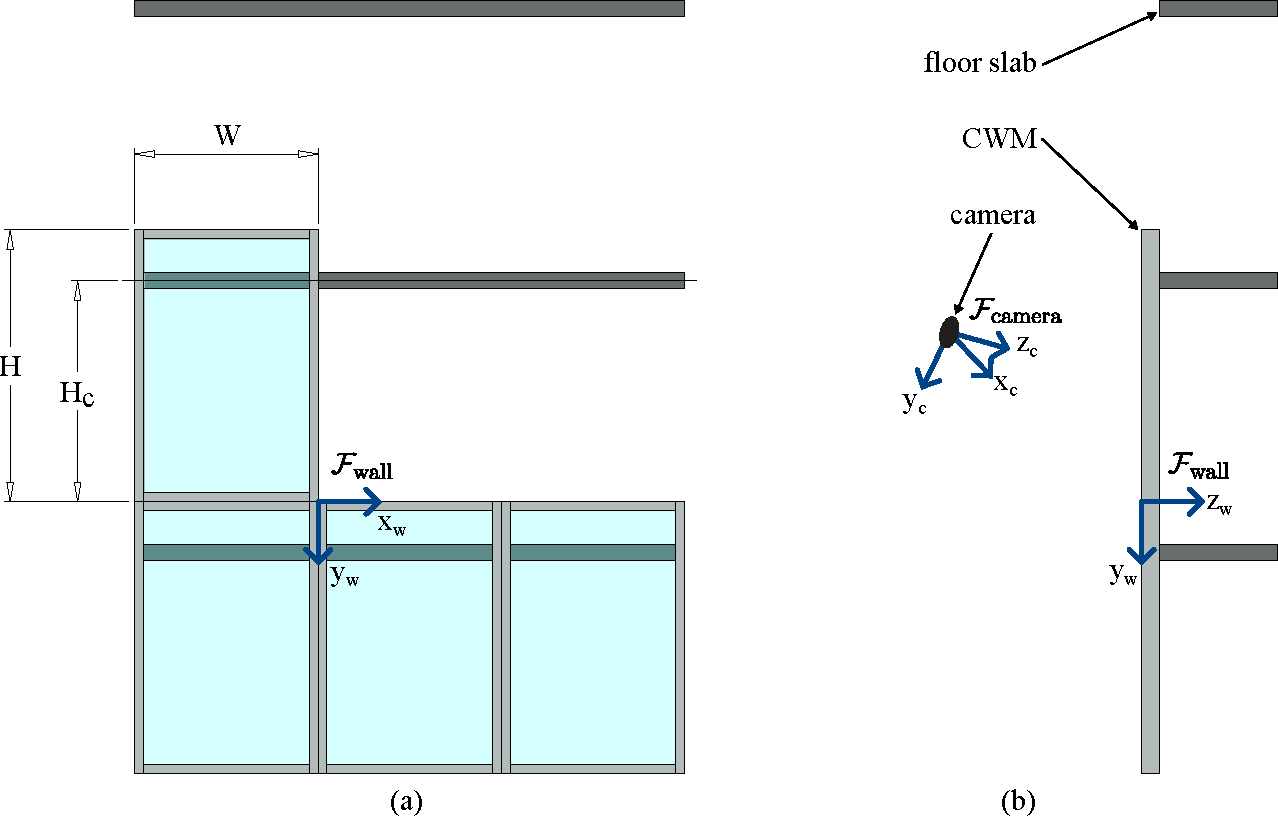
\includegraphics[width=\textwidth,keepaspectratio]{Figures/ExampleFigure3.pdf}}
	\caption{Export your graphics to pdf. Lovely vector graphics! If I see any jpeg text I am sad.}
	\label{fig:Example1}
\end{figure}

\begin{figure}[!htb]
	\centering
	\captionbox{Cool graphic!\label{fig:Example2}}
		[.5\textwidth]{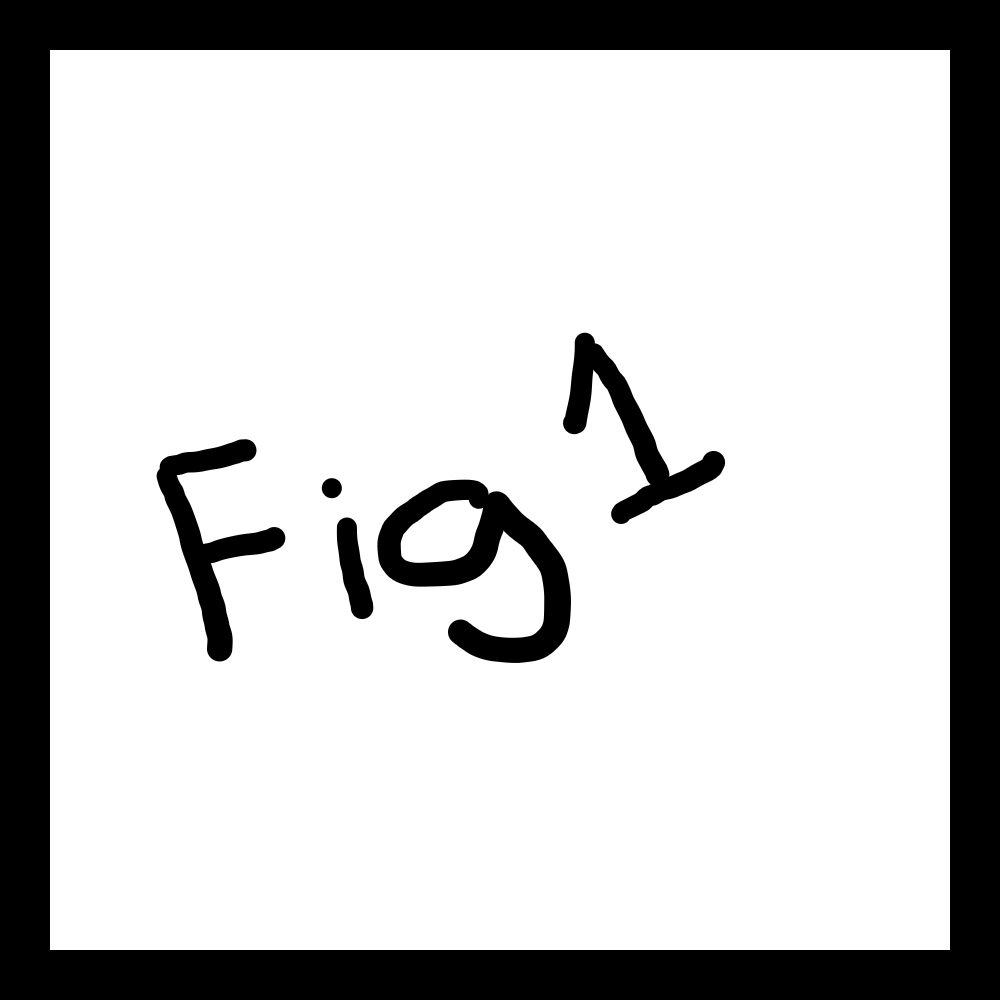
\includegraphics[width=0.5\textwidth,keepaspectratio]{Figures/ExampleFigure1.png}}%%
	\captionbox{This is a very long caption that takes up multiple lines.\label{fig:Example3}}
		[.5\textwidth]{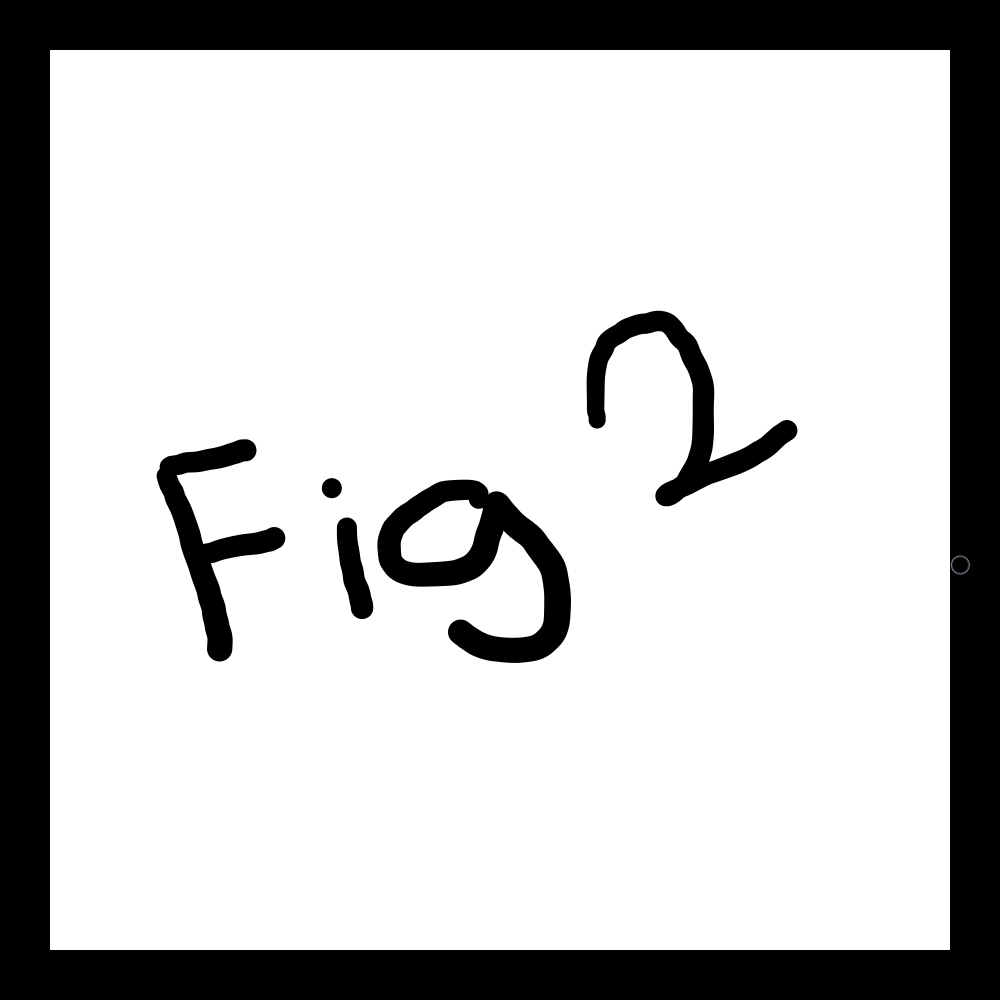
\includegraphics[width=0.5\textwidth,keepaspectratio]{Figures/ExampleFigure2.png}}
\end{figure}

\begin{figure}[!htb]
	\centering
    \begin{subfigure}[t]{0.49\textwidth}
        \centering
		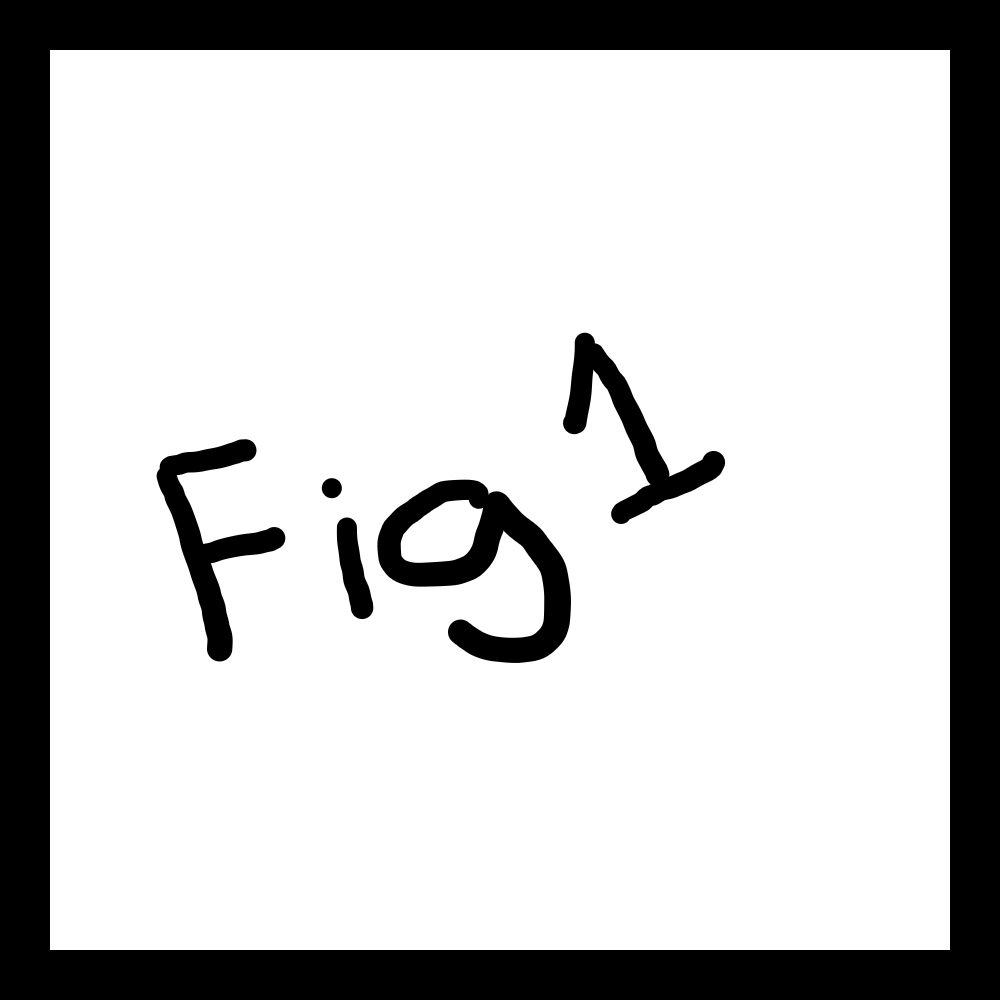
\includegraphics[width=\textwidth,keepaspectratio]{Figures/ExampleFigure1.png}
	    \caption{Cool graphic!}
        \label{fig:Example4a}
    \end{subfigure}
    \begin{subfigure}[t]{0.49\textwidth}
        \centering
		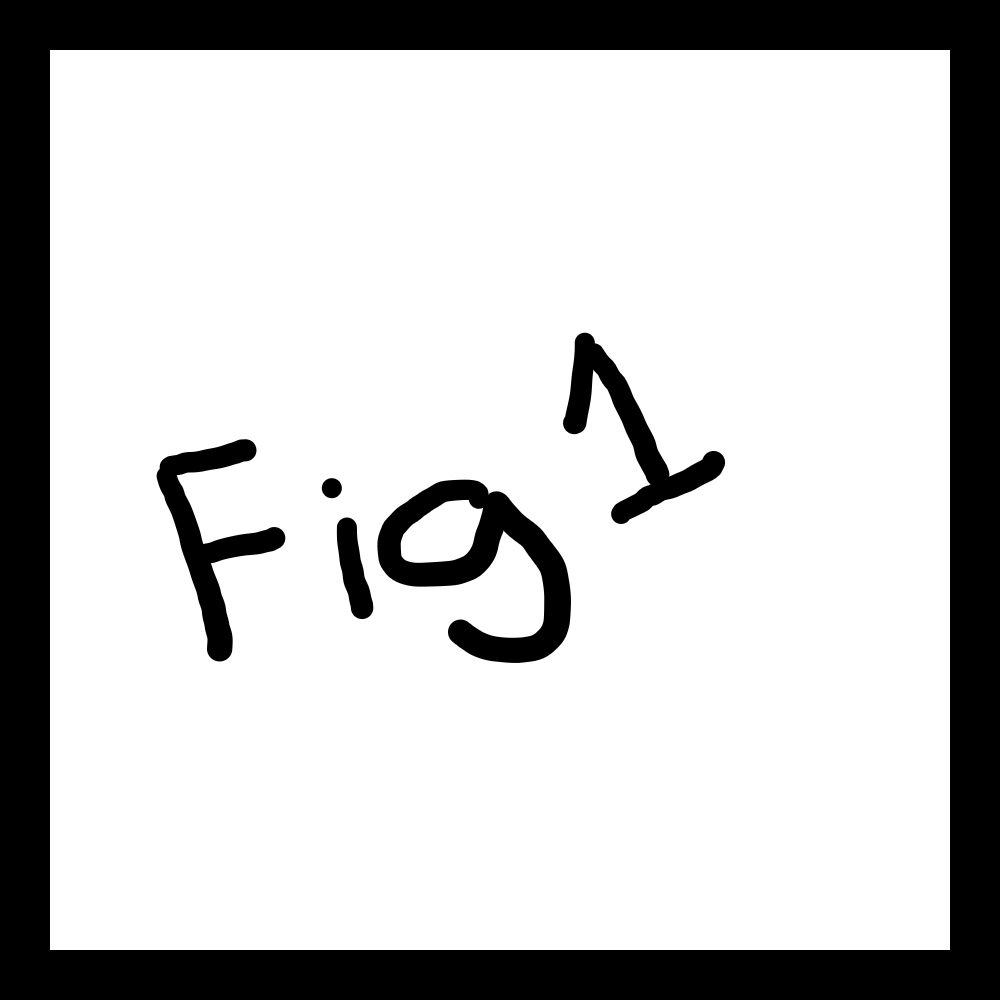
\includegraphics[width=\textwidth,keepaspectratio]{Figures/ExampleFigure1.png}
	    \caption{This is a very long caption that takes up multiple lines.}
        \label{fig:Example4b}
    \end{subfigure}
    \caption{Cool graphics!}
    \label{fig:Example4}
\end{figure}


%%%%%%%%%%%%%%%%%%%%%%%%%%%%%%%%%%%%%%%%%%%%%%%%%%%%%%%%%%%%%%%%%%%%%%%%%%%%%%%%%
\subsection{Equations}
This is an equation reference: \eqref{eq:myEq}.

\begin{equation} \label{eq:myEq}
    a = 2
\end{equation}

where $a$ is a variable.


%%%%%%%%%%%%%%%%%%%%%%%%%%%%%%%%%%%%%%%%%%%%%%%%%%%%%%%%%%%%%%%%%%%%%%%%%%%%%%%%%
\subsection{Tables}

This is a table reference: \tbref{tb:myTable}.

This is a fairly basic table. See threeparttable if you want table notes (footnotes for tables). For more fancy tables, use NiceTabular of the package NiceMatrix.

\begin{table}[!h]
    \centering
    \begin{tabular}{llll}
        \hline
        & & \multicolumn{2}{l}{Measurement error}\\
        Measurement & Unit & Mean & Standard deviation\\
        \hline
        $x_n$ & mm & 5.2 & 8.6\\
        $y_n$ & mm & 3.5 & 3.0\\
        $z_n$ & mm & -6.5 & 9.1\\
        $\theta_q$ & degrees & 1.6$\degree$ & 2.9$\degree$\\
        \hline
        \end{tabular}
    \caption{Average measurement error over all 99 successful measurements. $(x_n, y_n, z_n)$ are defined somewhere else. $\theta_q$ is the rotational misalignment as a quaternion angular distance.}
    \label{tb:myTable}
\end{table}


%%%%%%%%%%%%%%%%%%%%%%%%%%%%%%%%%%%%%%%%%%%%%%%%%%%%%%%%%%%%%%%%%%%%%%%%%%%%%%%%%
\subsection{Algorithms}

\begin{algorithm}
    \DontPrintSemicolon
    %% SYNTAX: \SetKwProg{CommandName}{Title}{ is}{end}
    \SetKwProg{Fn}{Function}{}{end}
    %% SYNTAX: \Set...{CommandName}{TextToDisplay}
    \SetKwFunction{Multiply}{Multiply}
    \SetKwInOut{TypeDefLength}{Length}
    \SetKwInOut{TypeDefArea}{Area}
    \SetKwIF{If}{ElseIf}{Else}{if}{}{else if}{else}{end} %% Actual IF statement (remove the "then")
    \SetKwIF{InputBlock}{}{}{Input}{}{}{}{end}{} %% Not an IF statement, just using the block structure
    \SetKwInOut{InputDefL}{$L$}
    \SetKwInOut{InputDefW}{$W$}
    %% START PRINTING
    \emph{Type Definitions}\\
    \TypeDefLength{A length measurement, with units in mm}
    \TypeDefArea{An area measurement, with units in $\text{mm}^\text{2}$}
    \BlankLine
    \nl \Fn{\Multiply}{
        %\ResetInOut{xx} %% This macro sets a fixed distance based on the text INSIDE IT..... WHY?
        \InputBlock{}{
            \InputDefL{[\KwSty{Length}] Object length}
            \InputDefW{[\KwSty{Length}] Object width}
        }
        \BlankLine
        \lnl{algo:M:vStart} \uIf{$L < 0$}{
            \lnl{algo:M:errorL} \KwRet{Bad input: L}
        }
        \nl \uElseIf{$W < 0$}{
            \lnl{algo:M:errorW} \KwRet{Bad input: W}
        }
        \nl \Else{
            \lnl{algo:M:vEnd} Carry on citizen\;
        }
        \lnl{algo:M:start} Copy $L$ into the calculator\;
        \lnl{algo:M:t} press the $\times$ button on the calculator\;
        \lnl{algo:M:w} Copy $W$ into the calculator\;
        \lnl{algo:M:e} Press the $=$ button on the calculator\;
        \lnl{algo:M:r} \KwSty{Area} $A \leftarrow$ The result shown on the calculator\;
        \BlankLine
        \lnl{algo:M:return} \KwRet{$A$, The area as measured in units of {\normalfont $\text{mm}^\text{2}$}}
    }
    \caption{Algorithm to find the area of an object.}
    \label{alg:myAlgo}
\end{algorithm}

Pseudocode of the  algorithm is \algoref{alg:myAlgo}. In the first stage of the algorithm, \algoRefLines{algo:M:vStart}{algo:M:vEnd} validate the inputs. Then \algoRefLines{algo:M:start}{algo:M:r} do the calculation. Then \algoRefLine{algo:M:return} outputs the result.

\chapter{Introduction}

\section{Writing a thesis}
Writing a thesis is a lengthy process, often requiring multiple redrafts and revisions.

Drafts should be provided and reviewed on a regular basis to keep up momentum as the submission deadline approaches. Please ensure that all required milestones and program requirements (e.g., professional development hours) have been completed before progressing with your submission.

The information below has been provided to you to make your experience as easy as possible. You may also like to refer to the Graduate Research Thesis Examination Procedures for further insight into the thesis examination process.

\subsection{What format the thesis will be presented}
The first thing to consider is in what format the thesis will be presented.
We recommend students and main supervisors discuss this as early as possible, and jointly agree on the most appropriate option:

Traditional thesis: A similar format to research reports and papers where the research question is proposed, methodology is described and the results are discussed and conclusions established.

Thesis including published works: Overall format is the same as a traditional thesis but particular chapters will include any submitted publications. Some Faculties have their own criteria for what can be included in this format.

All theses must use the approved thesis preliminary pages which includes compulsory information such as copyright and authorship declarations. If these pages are not presented correctly, the thesis will not be dispatched to the examiners and the relevant sections will need to be amended.

\subsection{Examiners}
At Monash each graduate research student has a supervisory team. Of this group, the main supervisor is responsible for approaching potential examiners for their students' thesis. Initial discussions normally take place at the student's final milestone review and it is recommended that examiners are approached at least 4-6 weeks before expected submission.

An email template is available for use when inviting potential examiners to examine a thesis.

For students enrolled in a Live Music or Theatre Performance degree, the main supervisor will also need to complete a Nomination of Examiners form. This form will require the approval of the Program Director (or delegate) and the Monash Graduate Research Office prior to the live performance. For further information please contact the Faculty of Arts.

In addition, when considering appropriate examiners, please note that if an examiner is subject to Sanctions laws, we are unable to provide payment for their thesis examination.

\subsection{Conflict of interest}
There are a range of circumstances that could result in a conflict of interest, potentially restricting the objectivity of the examiners.

Some examples of what we consider conflicts of interest are:
\begin{itemize}
\item Involvement in the student's research, including supervision of the candidate in field or laboratory work or elsewhere during candidature.
\item Previous work in the same department within an institution as the candidate.
\item A previous appointment as an academic staff member at Monash University, including an adjunct academic appointment, during the student’s period of candidature.
\item Holding the position of emeritus or adjunct professor at Monash.
\item Substantial contact with the candidate in any other circumstance which might jeopardise the independence of the examination.
\item Being a close associate (spouse/partner, other relative, friend or business partner) of either the candidate or the supervisor of the candidate.
\end{itemize}
There is a more comprehensive list of grounds for conflicts of interest which you may wish to review.


\section{Thesis including Published Works}
All doctoral and research master's students are permitted to submit a thesis including published works, in accordance with section 1.9 of the Graduate Research Thesis Examination Procedures. The thesis including published works is not a different degree; rather, it is a thesis format that includes papers that have been submitted, or accepted, for publication, during the course of the student's enrolment in the relevant graduate research degree at Monash.

The thesis must reflect a sustained and cohesive theme, and framing or substantial linking text is normally required in introducing the research and linking the chapter/papers/manuscripts. The papers do not have to be rewritten for the thesis. For guidance, refer to Text Framing the Publications (as below).

Whether the papers are required to have been published, accepted for publication, or only submitted for publication varies across faculties (see Faculty Requirements below). We advise you to consult good examples of theses including published works in your discipline. Your academic unit or school should have copies of all doctoral and research master's theses available for consultation. Workshops on the thesis including published works are also run through the Skills Essentials series, if you require more information.


\section{The maximum word length}
For references see \href{http://www.monash.edu/__data/assets/pdf_file/0011/911882/Graduate-Research-Thesis-Examination-Procedures.pdf}{Graduate Research Thesis Examination Procedures} 

PhD: 80,000 words,  100,000 words for students enrolled prior to 1 January 2015

MPhil: 35,000 words, 50,000 words for students enrolled prior to 1 January 2015.

\section{Using Figures and Tables, and other commands}

We have defined several commands in thesis.cls file for easier usage:
\begin{verbatim}
\newcommand{\fref}[1]{Figure~\ref{#1}}
\newcommand{\tref}[1]{Table~\ref{#1}}
\newcommand{\eref}[1]{Equation~\ref{#1}}
\newcommand{\cref}[1]{Chapter~\ref{#1}}
\newcommand{\sref}[1]{Section~\ref{#1}}
\newcommand{\aref}[1]{Appendix~\ref{#1}}
\renewcommand{\topfraction}{0.85}
\renewcommand{\bottomfraction}{.85}
\renewcommand{\textfraction}{0.1}
\renewcommand{\dbltopfraction}{.85}
\renewcommand{\floatpagefraction}{0.75}
\renewcommand{\dblfloatpagefraction}{.75}
\end{verbatim}

You can use \textit{fref} and \textit{tref} to refer a figure and table, such as \fref{fig.demo1} and \tref{table.demo1}. Refer a citation like this \cite{Reference1}. You can cite multiple references once, like this \cite{Reference1,Reference2,Reference3}.



\begin{figure}
\centering
  
\includegraphics[height=5cm]{Figures/crest.jpg}%
  \caption{My Picture Demo\label{fig.demo1}}
\end{figure}

\begin{table}[]
\caption{Table Demo.\label{table.demo1}}
\centering
\begin{tabular}{|c|c|c|}
\hline
Description & Images &  \\ \hline
Training & Taking 3 knowns + 1 known unknown randomly & 2900 \\ \hline
Gallery & Taking 3 images of knowns randomly & 1830 \\ \hline
Probe C & C=S & 4903 \\ \hline
Probe O1 & O1 & 6264 \\ \hline
Probe O2 & O2 & 8972 \\ \hline
Probe O3 & O3 & 10333 \\ \hline
\end{tabular}
\end{table}

\section{A Section}

Quisque tristique urna in lorem laoreet at laoreet quam congue. Donec dolor turpis, blandit non imperdiet aliquet, blandit et felis. In lorem nisi, pretium sit amet vestibulum sed, tempus et sem. Proin non ante turpis. Nulla imperdiet fringilla convallis. Vivamus vel bibendum nisl. Pellentesque justo lectus, molestie vel luctus sed, lobortis in libero. Nulla facilisi. Aliquam erat volutpat. Suspendisse vitae nunc nunc. Sed aliquet est suscipit sapien rhoncus non adipiscing nibh consequat. Aliquam metus urna, faucibus eu vulputate non, luctus eu justo.

\subsection{A Subsection}

Donec urna leo, vulputate vitae porta eu, vehicula blandit libero. Phasellus eget massa et leo condimentum mollis. Nullam molestie, justo at pellentesque vulputate, sapien velit ornare diam, nec gravida lacus augue non diam. Integer mattis lacus id libero ultrices sit amet mollis neque molestie. Integer ut leo eget mi volutpat congue. Vivamus sodales, turpis id venenatis placerat, tellus purus adipiscing magna, eu aliquam nibh dolor id nibh. Pellentesque habitant morbi tristique senectus et netus et malesuada fames ac turpis egestas. Sed cursus convallis quam nec vehicula. Sed vulputate neque eget odio fringilla ac sodales urna feugiat.

\section{Another Section}

Phasellus nisi quam, volutpat non ullamcorper eget, congue fringilla leo. Cras et erat et nibh placerat commodo id ornare est. Nulla facilisi. Aenean pulvinar scelerisque eros eget interdum. Nunc pulvinar magna ut felis varius in hendrerit dolor accumsan. Nunc pellentesque magna quis magna bibendum non laoreet erat tincidunt. Nulla facilisi.

Duis eget massa sem, gravida interdum ipsum. Nulla nunc nisl, hendrerit sit amet commodo vel, varius id tellus. Lorem ipsum dolor sit amet, consectetur adipiscing elit. Nunc ac dolor est. Suspendisse ultrices tincidunt metus eget accumsan. Nullam facilisis, justo vitae convallis sollicitudin, eros augue malesuada metus, nec sagittis diam nibh ut sapien. Duis blandit lectus vitae lorem aliquam nec euismod nisi volutpat. Vestibulum ornare dictum tortor, at faucibus justo tempor non. Nulla facilisi. Cras non massa nunc, eget euismod purus. Nunc metus ipsum, euismod a consectetur vel, hendrerit nec nunc.
\chapter{Including a published pdf as a thesis chapter}

In a thesis including published works, some chapters may simply involve including an external (published) \texttt{.pdf} file into your thesis document.

The following sample shows how to insert a subset of pages of a \texttt{.pdf} in such a way that the page numbering of the thesis is also added to the included \texttt{.pdf} pages. 
It also scales and translates the inserted \texttt{.pdf} file to fit within the margins of the thesis. 

% In the following command: 
% -- the argument {external} is the path to the pdf you would like to include (here the file happens to be called external.pdf and is in the Figures folder)
% -- the optional argument pages=1-2 inserts pages 1-2 of the referenced pdf (change this as required, for all pages write pages={-})
% -- the optional argument pagecommand={} keeps the overall page formatting of the thesis, including the overall page numbering
% -- the optional argument scale=0.85 scales the included pdf so it fits nicely on the thesis page (this may need to be altered depending on the margins of the pdf)
% -- the optinal argument offset=<x offset>mm <yoffset>mm specifies an offset from the nominal position. This will need to be adjusted so that the included document is placed well on the thesis page (i.e., margins are not violated, etc). In the example, the page is shifted 30mm to the right, and 20mm down (i.e., -20mm vertical offset). 
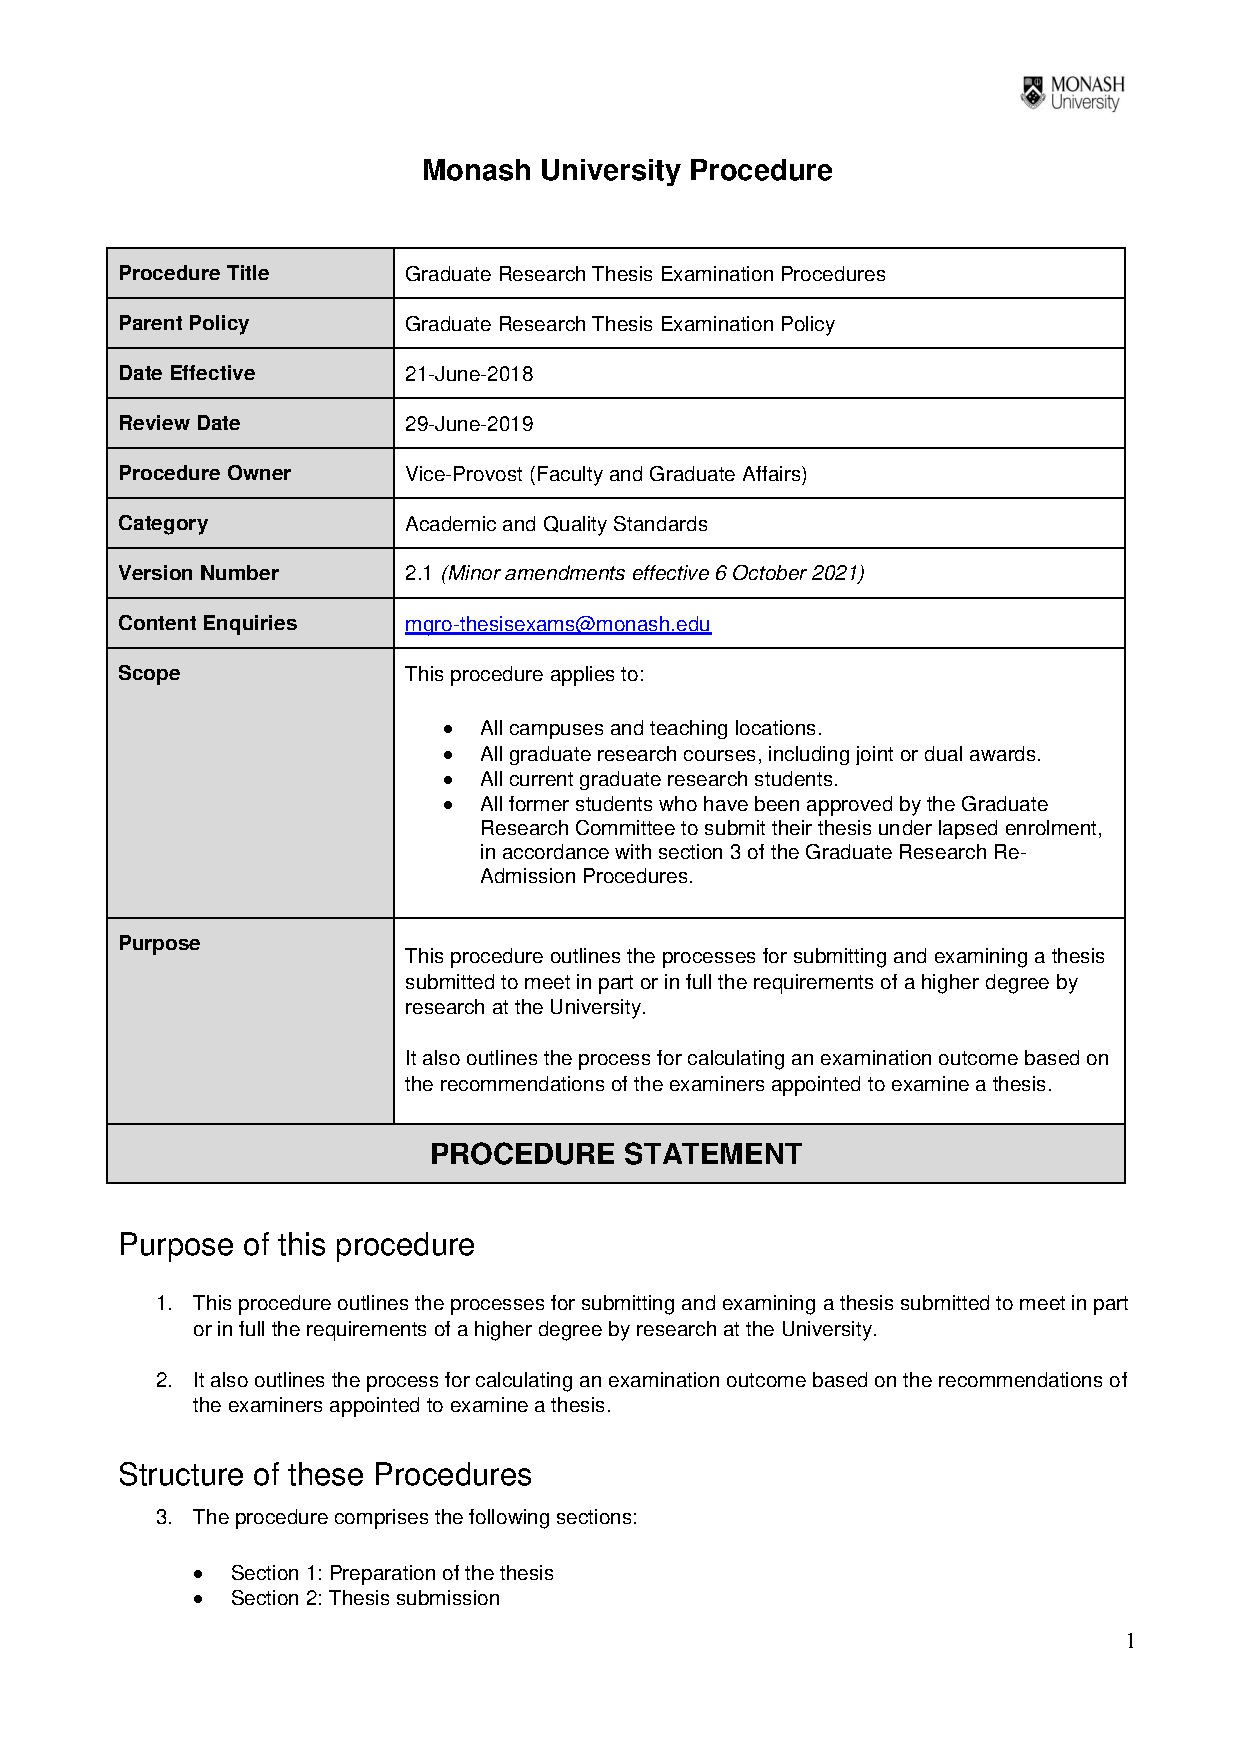
\includepdf[pages=1-2,pagecommand={},scale=0.85,offset=30mm -20mm]{Figures/external}
\chapter{My First Published Article} \label{chap:article1}
\begin{displayquote} \emph{%%
	This chapter embeds a copy of my publication \cite{example3}, which is distributed under the \href{https://creativecommons.org/licenses/by/4.0/}{Creative Commons CC BY 4.0 license}.
} \end{displayquote}

%% Intro & link to objectives



%%%%%%%%%%%%%%%%%%%%%%%%%%%%%%%%%%%%%%%%%%%%%%%%%%%%%%%%%%%%%%%%%%%%%%%%%%%%%%%%%
%%%%%%%%%%%%%%%%%%%%%%%%%%%%%%%%%%%%%%%%%%%%%%%%%%%%%%%%%%%%%%%%%%%%%%%%%%%%%%%%%
\section{The Title of My First Published Article}
List of Amendments to \cite{example3}
\begin{itemize}[topsep=0pt,beginpenalty=10000,first=\interlinepenalty10000]
	\item Equation 6 contains a typographical error, in which ${}^O\text{\textbf{p}}_i$ should be ${}^O\dot{\text{\textbf{p}}}_i$
\end{itemize}

%% The following embedded document represents your published article.
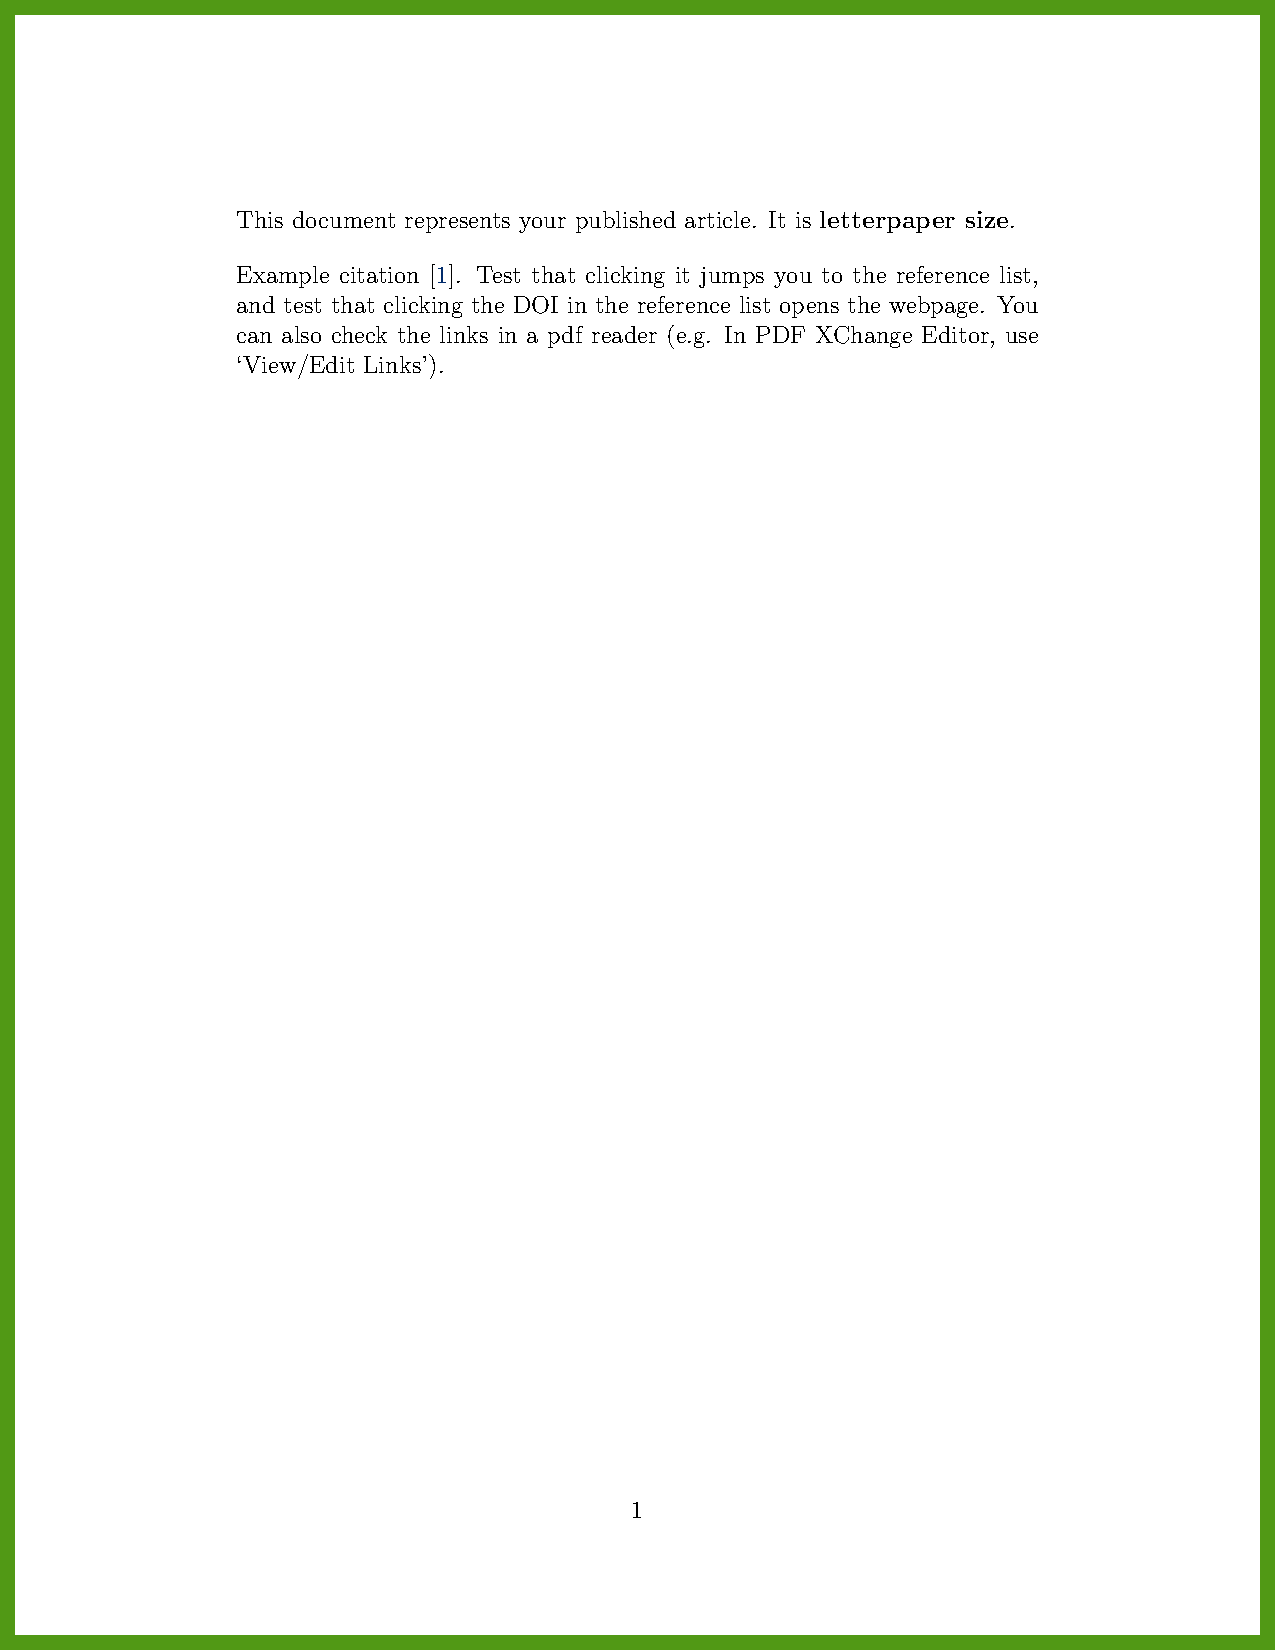
\includepdf[pages={-},pagecommand={},offset=0mm 10mm]{MyPublishedArticle1.pdf}

%% NOTE 1
%% The article is being embedded into an A4 document.
%% If the article is not A4, then it will be shrunk to fit and centred in the page.
%% The offset parameter can move from the default position
%% => If the thesis footer overlaps the included pdf, then try changing the scale and offset
%% e.g.
%% 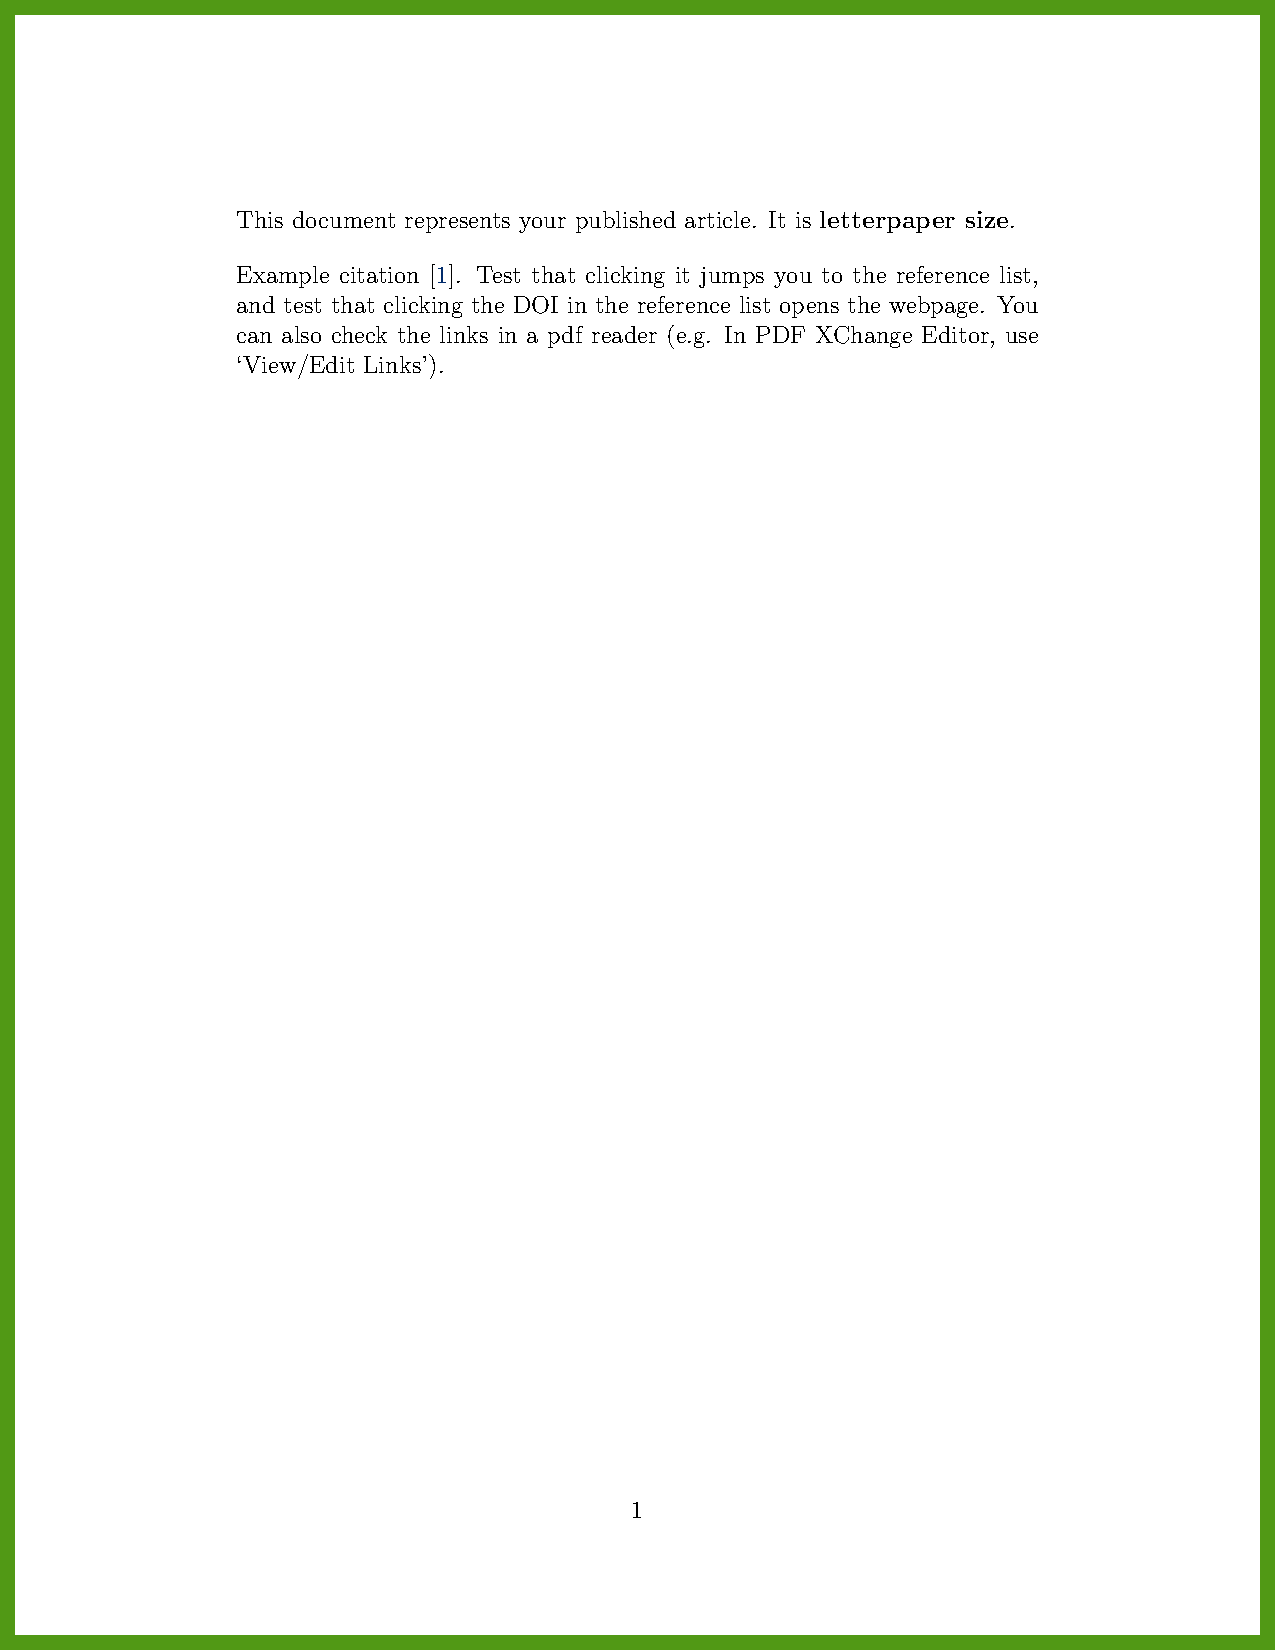
\includepdf[pages={-},pagecommand={},scale=0.95,offset=0mm 5mm]{MyPublishedArticle1.pdf}

%% NOTE 2
%% By using the package `pdfpages' to embed this pdf into the thesis, all the hyperlinks become no longer clickable.
%% To reinsert the links, the package `pax' can be used
%% Reinserting the links requires some manual work, and the `pax' is not flawless.
%% Follow the instructions in Thesis.tex, and be sure to test that it works.


%%%%%%%%%%%%%%%%%%%%%%%%%%%%%%%%%%%%%%%%%%%%%%%%%%%%%%%%%%%%%%%%%%%%%%%%%%%%%%%%%
%%%%%%%%%%%%%%%%%%%%%%%%%%%%%%%%%%%%%%%%%%%%%%%%%%%%%%%%%%%%%%%%%%%%%%%%%%%%%%%%%
\section{Outlook}
%% Link results to objectives
The outcomes of this work ...

The work finds that ...

The next chapter applies these results to ...


\chapter{My Second Published Article} \label{chap:article2}
\begin{displayquote} \emph{%%
	This chapter embeds a copy of my publication \cite{example5}, which is distributed under the \href{https://creativecommons.org/licenses/by/4.0/}{Creative Commons CC BY 4.0 license}.
} \end{displayquote}

%% Intro & link to objectives



%%%%%%%%%%%%%%%%%%%%%%%%%%%%%%%%%%%%%%%%%%%%%%%%%%%%%%%%%%%%%%%%%%%%%%%%%%%%%%%%%
%%%%%%%%%%%%%%%%%%%%%%%%%%%%%%%%%%%%%%%%%%%%%%%%%%%%%%%%%%%%%%%%%%%%%%%%%%%%%%%%%
\section{The Title of My Second Published Article}
%% If the footer overlaps the included pdf, then try changing the scale and offset options e.g.
%% 
\includepdf[pages={-},pagecommand={},scale=0.95,offset=0mm 5mm]{MyPublishedArticle2.pdf}


\includepdf[pages={-},pagecommand={}]{MyPublishedArticle2.pdf}


%%%%%%%%%%%%%%%%%%%%%%%%%%%%%%%%%%%%%%%%%%%%%%%%%%%%%%%%%%%%%%%%%%%%%%%%%%%%%%%%%
%%%%%%%%%%%%%%%%%%%%%%%%%%%%%%%%%%%%%%%%%%%%%%%%%%%%%%%%%%%%%%%%%%%%%%%%%%%%%%%%%
\section{Outlook}
%% Link results to objectives
The outcomes of this work ...



\chapter{Conclusions and Outlook} \label{chap:conclusions}
%% Scope / Motivations / Problem Statement

%% Aims
%% Contributions as dot points
This thesis contributes to ... The key contributions are:
\begin{itemize}[topsep=0pt,beginpenalty=10000,first=\interlinepenalty10000]
	\item Something
	\item Something
	\item Something
\end{itemize}

%% Results and outlook
The outcomes of this work ...:
\begin{itemize}[topsep=0pt,beginpenalty=10000,first=\interlinepenalty10000]
	\item In \chapref{chap:article1}, it is found that ...
	\item In \chapref{chap:article2}, ...
\end{itemize}

%% Directions
Future work is recommended to ... Specific directions for future work are:
\begin{itemize}[topsep=0pt,beginpenalty=10000,first=\interlinepenalty10000]
	\item Something
	\item Something
	\item Something
\end{itemize}


\clearpage %% Start a new page


%%%%%%%%%%%%%%%%%%%%%%%%%%%%%%%%%%%%%%%%%%%%%%%%%%%%%%%%%%%%%%%%%%%%%%%%%%%%%%%%%
%%%%%%%%%%%%%%%%%%%%%%%%%%%%%%%%%%%%%%%%%%%%%%%%%%%%%%%%%%%%%%%%%%%%%%%%%%%%%%%%%
%% Header/footer style
\appendix
\assignpagestyle{\chapter}{appfirst}
\pagestyle{app}
\renewcommand{\chaptermark}[1]{ \markboth{\ $\vert$\ #1}{\thesubsection} }
\renewcommand{\sectionmark}[1]{ \markright{\thesubsection} }
\renewcommand{\subsectionmark}[1]{ \markright{\thesubsection} }
\renewcommand{\subsubsectionmark}[1]{}
\renewcommand{\paragraphmark}[1]{}
\renewcommand{\subparagraphmark}[1]{}

%% ACTION
%%      Add you content to the appendices
%%      Delete any unused chapters
%%      If you have no appendices, it is sufficient to delete only the \input{} lines
\chapter{An Appendix}
Example text.

%%%%%%%%%%%%%%%%%%%%%%%%%%%%%%%%%%%%%%%%%%%%%%%%%%%%%%%%%%%%%%%%%%%%%%%%%%%%%%%%%
%%%%%%%%%%%%%%%%%%%%%%%%%%%%%%%%%%%%%%%%%%%%%%%%%%%%%%%%%%%%%%%%%%%%%%%%%%%%%%%%%
\section{Displaying Sections}
Example text.

\clearpage

%%%%%%%%%%%%%%%%%%%%%%%%%%%%%%%%%%%%%%%%%%%%%%%%%%%%%%%%%%%%%%%%%%%%%%%%%%%%%%%%%
\subsection{My Subsection}
Example text.


%%%%%%%%%%%%%%%%%%%%%%%%%%%%%%%%%%%%%%%%%%%%%%%%%%%%%%%%%%%%%%%%%%%%%%%%%%%%%%%%%
\subsubsection{My Subsubsection}
Example text.

\clearpage

%%%%%%%%%%%%%%%%%%%%%%%%%%%%%%%%%%%%%%%%%%%%%%%%%%%%%%%%%%%%%%%%%%%%%%%%%%%%%%%%%
\paragraph{My Subsubsubsection... WAIT WHAT!?}
If you get this deep, the command is not `subsubsubsection', but `paragraph'. Why?

For the record, I really suggest not to use this much depth unless you've really thought about your structure, and you are sure that it is the best way to do it.

%%%%%%%%%%%%%%%%%%%%%%%%%%%%%%%%%%%%%%%%%%%%%%%%%%%%%%%%%%%%%%%%%%%%%%%%%%%%%%%%%
\subparagraph{My Subsubsubsubsection... rofl}
This is the maximum section depth that the titlesec package allows. May you never need it.


%%%%%%%%%%%%%%%%%%%%%%%%%%%%%%%%%%%%%%%%%%%%%%%%%%%%%%%%%%%%%%%%%%%%%%%%%%%%%%%%%
\subsection{My Other Subsection}
Example text.


\chapter{Another Appendix}
todo

\clearpage %% Start a new page


%%%%%%%%%%%%%%%%%%%%%%%%%%%%%%%%%%%%%%%%%%%%%%%%%%%%%%%%%%%%%%%%%%%%%%%%%%%%%%%%%
%%%%%%%%%%%%%%%%%%%%%%%%%%%%%%%%%%%%%%%%%%%%%%%%%%%%%%%%%%%%%%%%%%%%%%%%%%%%%%%%%
%% Header/footer style
\backmatter
\assignpagestyle{\chapter}{bibfirst}
\pagestyle{bib}

\label{Bibliography}
\printbibliography


%%%%%%%%%%%%%%%%%%%%%%%%%%%%%%%%%%%%%%%%%%%%%%%%%%%%%%%%%%%%%%%%%%%%%%%%%%%%%%%%%
%%%%%%%%%%%%%%%%%%%%%%%%%%%%%%%%%%%%%%%%%%%%%%%%%%%%%%%%%%%%%%%%%%%%%%%%%%%%%%%%%
\end{document}
